\chapter{Simulation}

%--------------------------------------------------------------------------------------------------------
% 		Intro
%--------------------------------------------------------------------------------------------------------
\section{Intro}

In this section, we create realistic scenarios that model the environments of some of its applications.  
For example, the random movement of a mobile phone user a car moving at varying speeds around source nodes.  
By examining the performance evaluations of the message ferrying design using parametric studies., it can predict how it will perform in its different environments and applications.
The varying speed of a car is taken into consideration in the network models and the random movement of mobile phone users.
These and among other varied parameters are explained in section \ref{sec:metrics}.

%More realistic scenario
%	- Random ferry movement
%		- Details -> car
%	- even source spacing

%--------------------------------------------------------------------------------------------------------
% 		Topology
%--------------------------------------------------------------------------------------------------------
\section{Network Model}

In this section, the two network models will be explained.
Their difference lies on the number of ferry, gateway, and source nodes.
And 
Their common settings are explained in section \ref{sec:commonsettings}.

%Might not need subsections for Scenario 1 & 2

\subsection{Scenario 1}		%1 gateway, 1 ferry
This scenario has one gateway, one ferry node, and ten source nodes.
The gateway is placed in the center and the ferry node starts next to it.
%picture of the scenario2 (1f1g random movement)
\begin{figure}[ht]
    \centering
    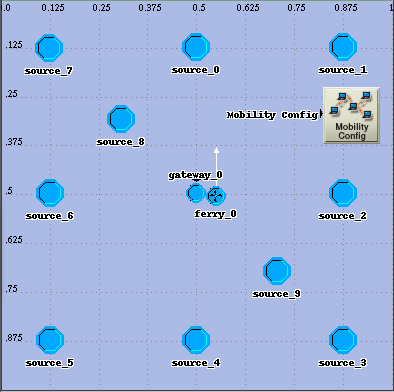
\includegraphics[width=.5\textwidth]{images/scenario2-top}
    \caption{Topology of Scenario 2}
    \label{fig:scenario2}
\end{figure}


\subsection{Scenario 2}		%2 gateways, 2 ferries
This scenario has two gateways and two ferry nodes. 
The gateways are placed near the center, while both ferries start from the center.
The distance between source nodes and the gateways are spaced evenly.
%picture of the scenario3 (2f2g random movement)
\begin{figure}[ht]
    \centering
    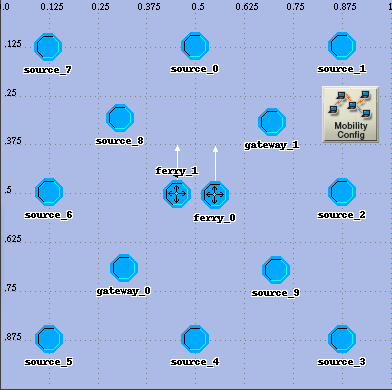
\includegraphics[width=.5\textwidth]{images/scenario3-top}
    \caption{Topology of Scenario 3}
    \label{fig:scenario3}
\end{figure}


\subsection{Common Settings}
\label{sec:commonsettings}
Some of the settings and characteristics common to all the topologies are the following:
\begin{itemize}
	\item All ferries move in random directions and have a varying speeds of 36kph - 72kph in uniform distribution 
	\item The size of all topologies is 1km x 1km
	%\item Beaconing intervals  %TO DO
	\item Property update interval of every 2s and a variance of 0.1s
	\item Simulations were run for 90 minutes. Property updates were disabled for the last thirty minutes in an effort to obtain statistics valid for a simulation of indefinite length. 
\end{itemize}


%--------------------------------------------------------------------------------------------------------
% 		Metrics and Results of Interest 
%--------------------------------------------------------------------------------------------------------
\section{Metrics and Results of Interest }
\label{sec:metrics}

%Some introduction
The metrics used are success rate and loss, delay, parameters  %TO DO

\subsection{Success Rate and Loss}
\label{sec:packetloss}
Because of the nature of the message ferrying algorithm, there may be dropped packets when the update number is older.
Those dropped packets are not to be accounted for packet loss because it is part of the algorithm`s process.
So, the packet loss is defined as where it measures the number of packets dropped when the buffer is full, where oldest packets are dropped to accommodate for adding the new packet.
The packet success rate is simply one minus the packet loss function with respect to the memory limit.

%Result of Interest 1: Success rate
%	- Main parameter of interest affecting success rate -> memory size
%	- Need to talk about what constitutes success rate

\subsection{Delay}
\label{sec:delay}
The delay is defined by the time to update the central repository once the update packet is sent out.  
The parameter affecting this delay is the number of ferries and gateways.
%Something about delay for lost packets

\subsection{Parameters Varied} %TODO: better section title
The following parameters are varied to obtain results for the metrics mentioned before in section \ref{sec:delay} and \ref{sec:packetloss}.
  
\subsubsection{Memory Limit}
The memory limit is the buffer size limit used.
It sets the maximum number of packets to handle.  

\subsubsection{Number of Ferries and Gateways}
The increase of the number of gateways reduced the delay of updating to central repository.  
This result was expected because we knew that by properly placing another gateway in the area will grant better coverage.  

\subsubsection{Seed - Effect of Randomness}
The different seeds used in the simulation results affect the randomness of movement.  

\subsubsection{Source Node Storage}
\label{sec:source_node_storage}
This is an option that allows the source nodes to be able to store update packets for the ferry nodes, which will then provide better ranges of transfer.
